\section{Frontend de la aplicación}

El frontend ha sido desarrollado como una aplicación web moderna y responsiva, utilizando las últimas tecnologías del ecosistema React. En esta sección, se presentan las diferentes tecnologías que han intervenido en el desarrollo de esta pieza de software, la arquitectura que sigue el proyecto de frontend, las diferentes páginas que lo componen, y varias técnicas de optimización que se han empleado.


\subsection{Stack Tecnológico}

La aplicación se ha construido utilizando el siguiente stack tecnológico:

\begin{itemize}
    \item React 19: Biblioteca principal para la construcción de interfaces de usuario basadas en componentes.
    \item Next.js 15: Framework de React que proporciona renderizado del lado del servidor (SSR), enrutamiento basado en archivos y optimizaciones de rendimiento automáticas.
    \item TypeScript: Superset tipado de JavaScript que proporciona seguridad de tipos en tiempo de compilación.
    \item Tailwind CSS: Framework de CSS utility-first para un desarrollo de estilos rápido y consistente. El uso este librería agiliza la aplicación de interfaces responsivas, adaptándose a todo tipo de dispositivos con tamaños de pantalla diversos.
    \item Framer Motion: Biblioteca de animaciones para crear transiciones fluidas y experiencias interactivas.\cite{framer_motion_docs}
    \item React Quill: Editor de texto enriquecido basado en Quill.js para la escritura de cartas.\cite{quill_react_playground}
    \item Axios: Cliente HTTP para comunicación con la API backend.
    \item React Leaflet: Biblioteca para integración de mapas interactivos.\cite{react_leaflet_docs}
\end{itemize}

\subsection{Arquitectura del Frontend y Gestión del Estado}

El proyecto sigue la estructura de \textit{App Router} de Next.js 13+, que organiza las rutas de la aplicación en función de la estructura de directorios. La estructura consta de las siguientes capas:

\begin{itemize}
    \item \texttt{app/}: Directorio principal que contiene las páginas y rutas de la aplicación. Cada subcarpeta se convierte en una ruta de la web automáticamente si incluimos dentro un archivo \texttt{page.tsx}.
    \item \texttt{components/}: Componentes reutilizables de la interfaz de usuario.
    \item \texttt{services/}: Capa de servicios que encapsula las llamadas a la API.
    \item \texttt{context/}: Contextos de React para gestión de estado global.
    \item \texttt{lib/}: Utilidades, tipos de TypeScript y constantes.
    \item \texttt{stylesheets/}: Aunque los estilos se aplican mayoritariamente con Tailwind CSS, para ciertos casos se utilizan estilos personalizados complementarios compartidos por varios componentes.
\end{itemize}


Para facilitar la escalabilidad y la reutilización del código, se han desarrollado \textbf{componentes reutilizables} para encapsular elementos como botones, inputs, selectores, descripciones emergentes, etc. Estos se incluyen en diferentes páginas y componentes de la aplicación para garantizar patrones de diseño consistentes, evitar la duplicación de lógica, y facilitar la implementación de cambios globales.

En cuanto a la \textbf{comunicación con el backend}, la capa de servicios encapsula toda la lógica de acceso a la API, que se implementa con Axios. La capa incluye cuatro módulos diferenciados por funcionalidad: usuarios, cartas, correcciones y amistades. Cada módulo de servicio exporta funciones asíncronas que manejan configuración de headers de autenticación, errores HTTP y de Axios, transformación de datos entre el formato de la API y el formato esperado por los componentes; y validación básica de datos antes del envío.

Respesto a la gestión del estado de la aplicación, se deben almacenar ciertos datos comunes a todas o varias páginas, así como datos individuales de cada página o componente. Para ello, se utilizan múltiples estrategias:

\begin{itemize}
    \item \textbf{Local Storage}: Utilizado para datos no sensibles de la experiencia de usuario, como la preferencia de tema (modo claro u oscuro), que se establece inicialmente como el que tenga por defecto el usuario en su navegador, pero puede ser configurarse desde el menú desplegable de Letterex.
    \item \textbf{React Hooks}: Se usan funciones especiales de React como \texttt{useState}, \texttt{useEffect} o \texttt{useRef}, para controlar el estado local de los componentes. Este último se usa para implementar una caché en memoria por página, por ejemplo, guardando resultados paginados. Cuando el usuario vuelve a una página ya consultada, los datos se leen desde caché y se muestran al instante. Así, se consigue una mejora del rendimiento por la reducción de llamadas redundantes al servidor.
    \item \textbf{Context API}: guarda el estado del componente para gestionar diálogos modales de forma centralizada, evitando \textit{prop drilling}, fenónemo en que los componentes se pasan datos de padres a hijos sucesivamente quedando varios hijos intermedios que no los utilizan. Con un proveedor de contexto, la app es capaz de renderizar un solo componente de diálogo que se abre y se cierra con dos funciones a las que cualquier componente puede acceder fácilmente, en este caso mediante un hook personalizado llamado \texttt{useDialog} que devuelve el contexto del diálogo. Por ejemplo, la siguiente figura muestra la función que abrirá el diálogo de error a su derecha. Esta estrategia se utiliza también para guardar los datos no sensibles del usuario autenticado.

    \begin{figure}[H]
        \centering
        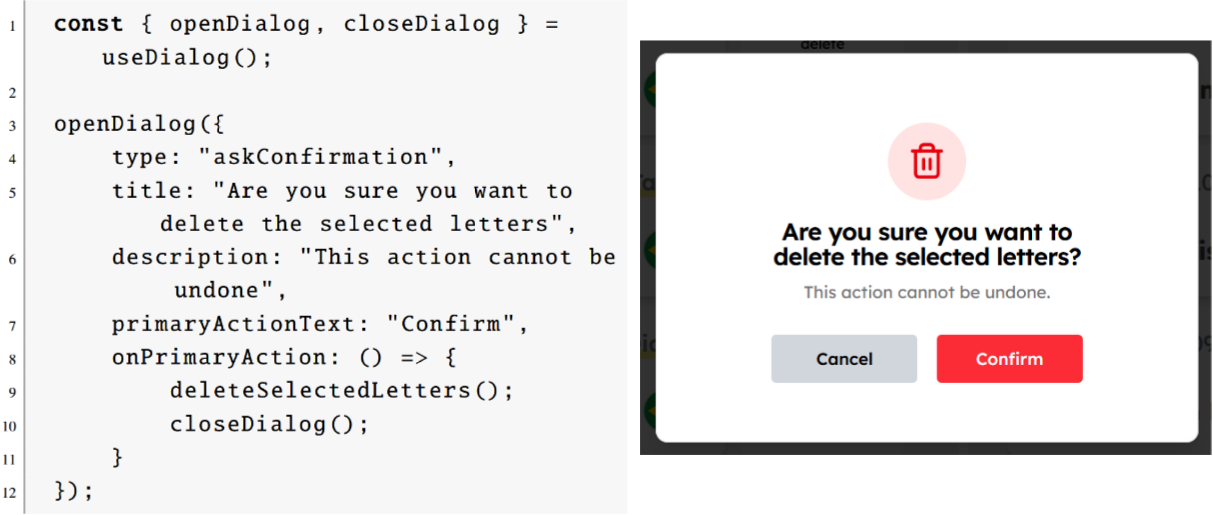
\includegraphics[width=\textwidth]{imagenes/ui/dialogDeleteAll.png}
        \caption{Código de apertura del diálogo y resultado en la interfaz}
        \label{fig:dialog}
    \end{figure}

\end{itemize}



\subsection{Páginas de la aplicación}

En este apartado se irán mostrando las diferentes páginas que componen la interfaz, que en total son siete: la página de inicio de sesión, la página principal, la página para la creación de una nueva carta, la página de correción de cartas recibidas, la página de visualización de una correción recibida, la página de amigos, y la página de perfil de usuario.

En las paginas protegidas (aquellas a las que se accede tras iniciar sesión), el componente \texttt{Sidebar} envuelve todo el contenido para proporcionar una barra lateral de navegación persistente con acceso rápido a todas las páginas de la aplicación.

\subsubsection{Página de Inicio y Autenticación}

\begin{figure}[h]
    \centering
    
\includegraphics[width=\textwidth]{imagenes/ui/login.png}
    \caption{Página de inicio de sesión y registro}
    \label{fig:landing}
\end{figure}

La página de inicio presenta una interfaz atractiva y animada que da la bienvenida a los usuarios. Esta página utiliza el componente \texttt{AnimatedForm} que gestiona tres estados principales:

\begin{itemize}
    \item \textbf{Bienvenida}: Presenta el propósito de la aplicación con un efecto de escritura animado (\textit{typewriter}) que muestra frases como ``Write about your passions'', ``Exchange language corrections'' y ``Find people to share and learn'', para dar una idea general de aquello en que consiste la plataforma.
    \item \textbf{Inicio de sesión}: Formulario de inicio de sesión para usuarios existentes.
    \item \textbf{Registro}: Formulario de registro con verificación de email mediante el código enviado a su correo, selección de idioma nativo e idiomas de interés, selección de contraseña y nombre de usuario, y posibilidad de subir una foto de perfil.
    \item \textbf{Olvido de contraseña}: Formulario que permite resetear la contraseña del usuario mediante el código de verificación enviado a su email.
\end{itemize}

Una característica distintiva de esta página es la animación del logo implementada con Framer Motion, que se desplaza suavemente entre diferentes posiciones según el formulario activo, proporcionando un elemento lúdico y memorable a la experiencia del usuario.
\subsubsection{Página Principal}

\begin{figure}[h]
    \centering
    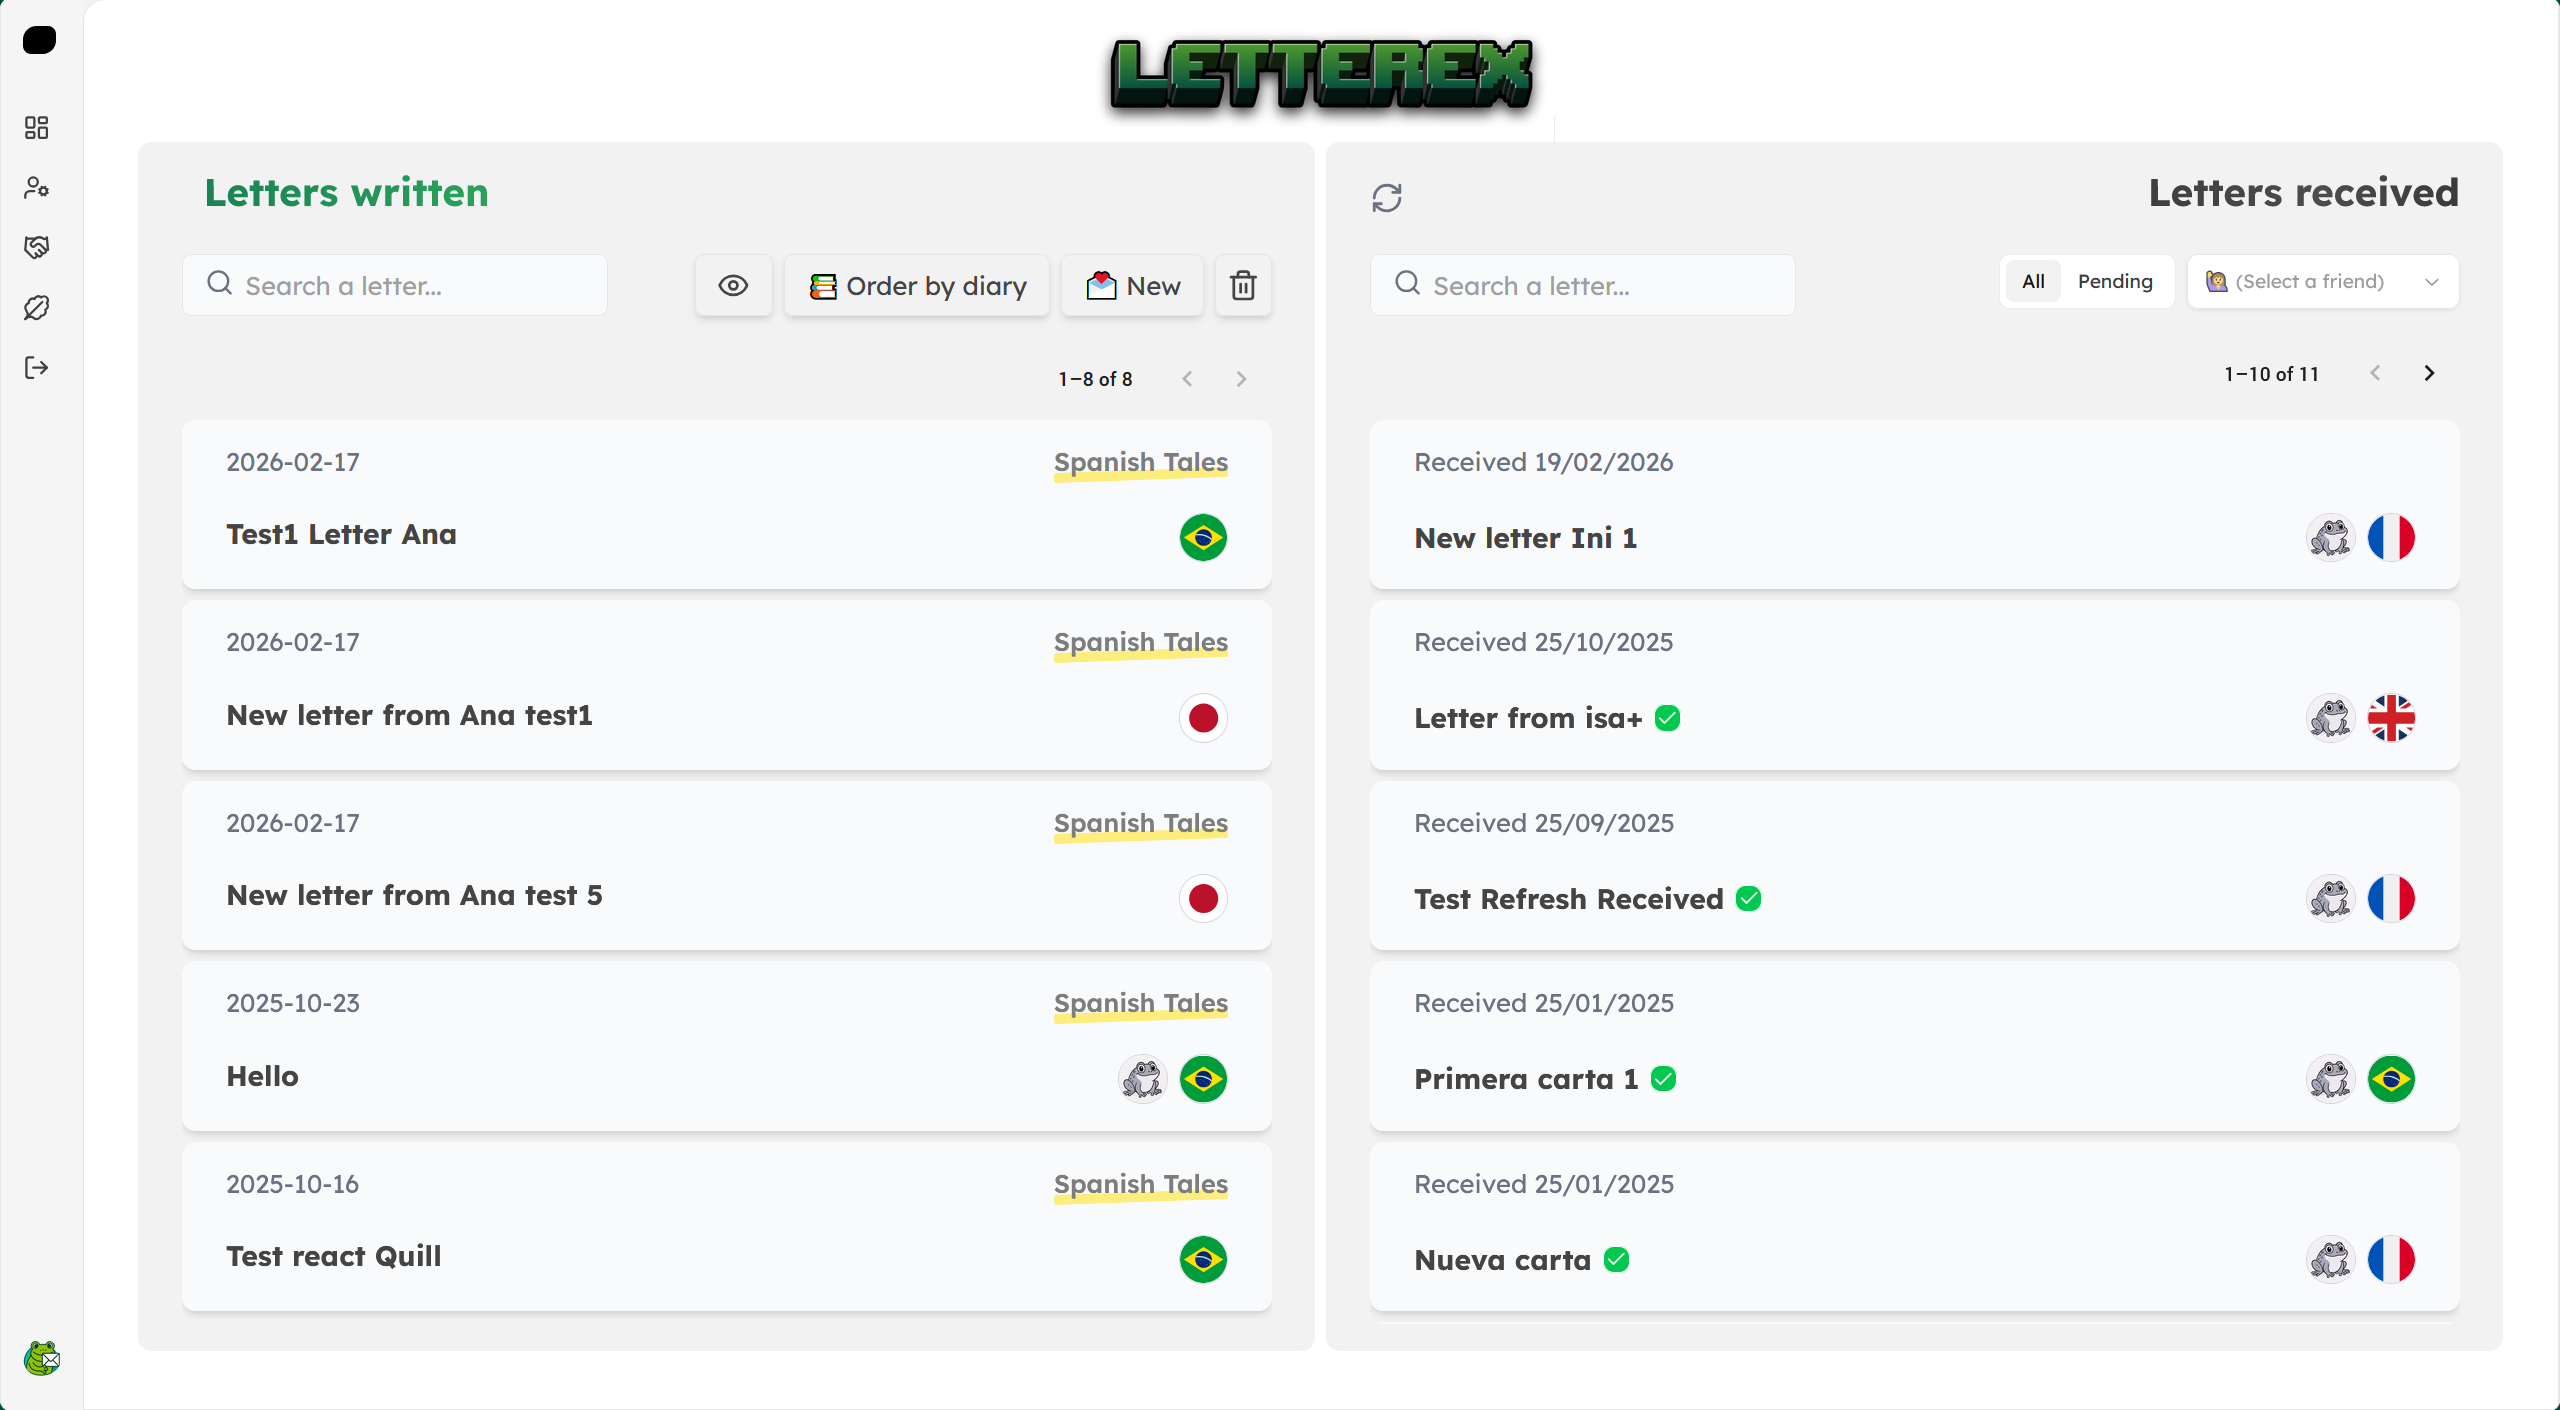
\includegraphics[width=\textwidth]{imagenes/ui/homepage.png}
    \caption{Página principal}
    \label{fig:homepage}
\end{figure}

El dashboard principal (\texttt{/homepage}) es la página central de la aplicación después del inicio de sesión. Está estructurado en dos secciones principales:

\begin{enumerate}
    \item \textbf{Letters Written}: Muestra las cartas que el usuario ha escrito, organizadas en tarjetas interactivas con un efecto de desliz que revela información adicional al interactuar, y paginadas en tandas de 5 elementos. Permite filtrar por una búsqueda, ordenar las cartas por diarios, y eliminar una o varias cartas de la lista. Clicando en la tarjeta de una carta se accede a la página de visualización o edición de esta, clicando en la tarjeta de usuario corrector que aparece al \textit{hover} (posar el cursor sobre el elemento) se accede a la página de visualización de corrección en caso de haberla, y clicando en el botón \textit{New} de la barra de herramientas se accede a la página para crear una nueva carta.
    \item \textbf{Letters Received}: Presenta las cartas recibidas de usuarios que solicitan una corrección por parte del usuario actual, paginadas de la misma forma que las anteriores. Permite filtrar por una búsqueda, por usuario que envió la carta, y por si esa carta está pendiente de corregir (no fue corregida y enviada de vuelta todavía). Clicando en la tarjeta de una carta recibida, se accede a la página de correción de dicha carta.
\end{enumerate}

\subsubsection{Páginas de Creación y Edición de Cartas}

\begin{figure}[h]
    \centering
    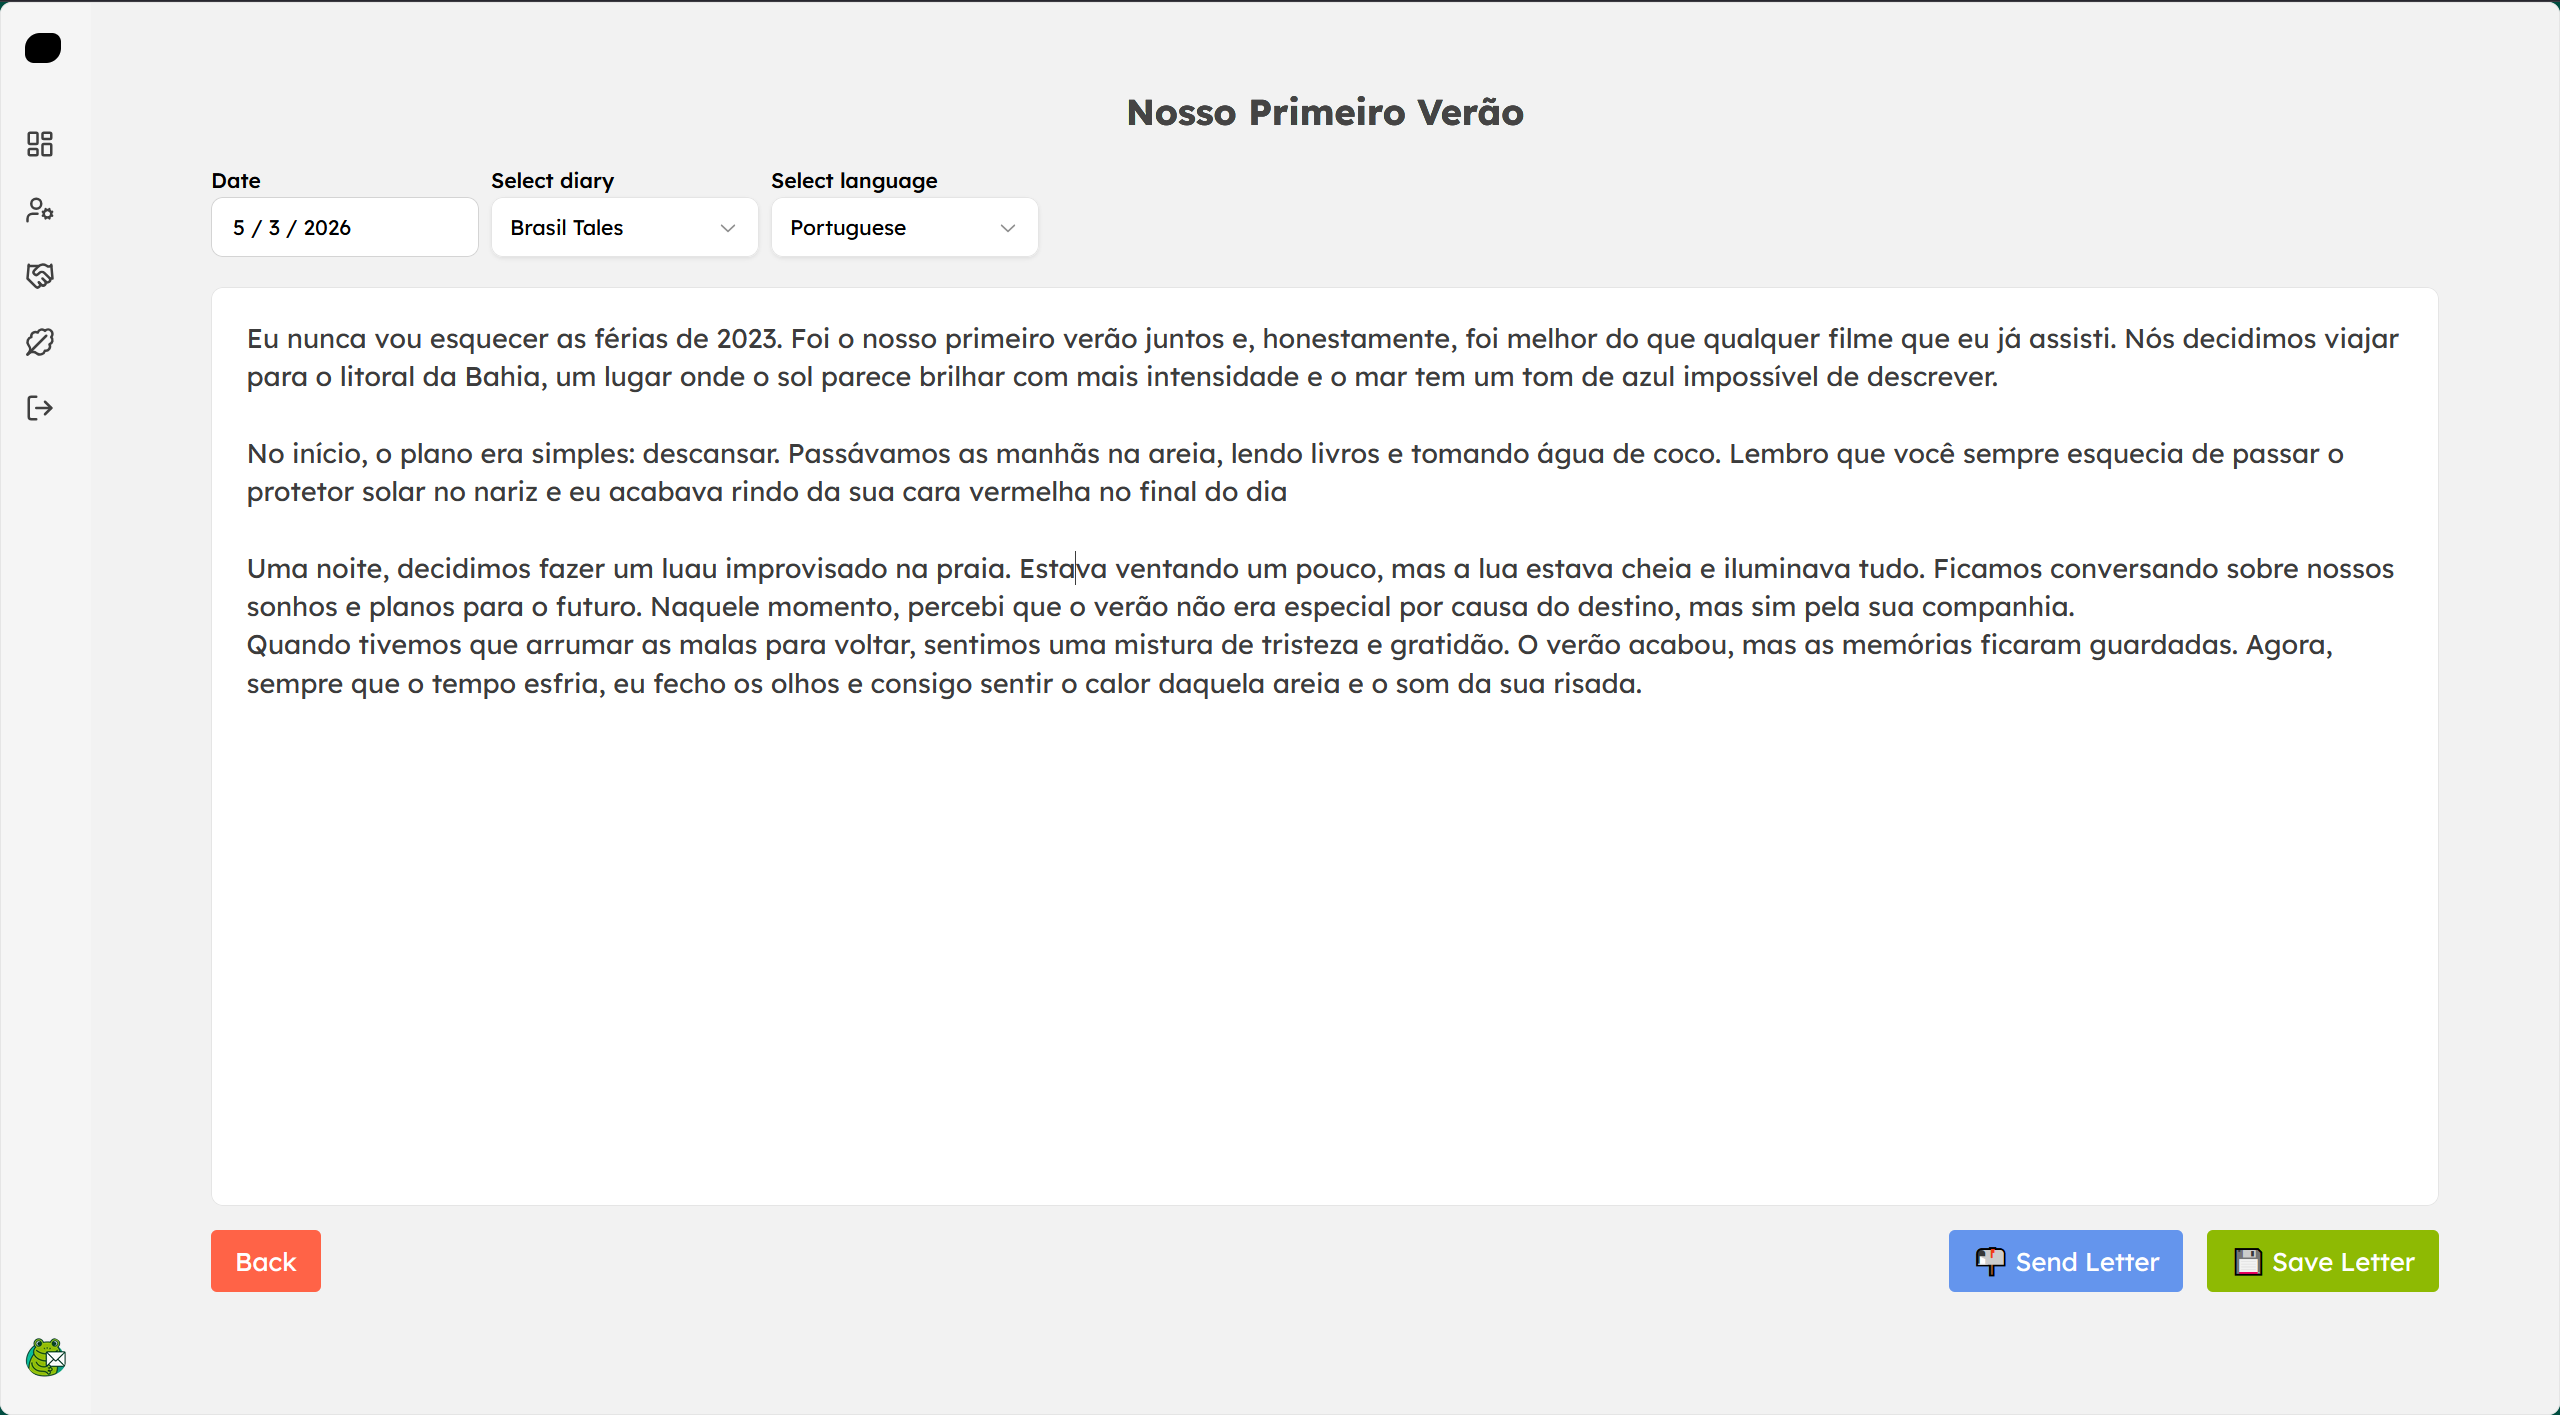
\includegraphics[width=\textwidth]{imagenes/ui/new-letter.png}
    \caption{Página de creación de cartas}
    \label{fig:new-letter}
\end{figure}

La página de creación de cartas (\texttt{/new-letter}) proporciona una interfaz completa para escribir nuevas entradas de diario. El componente implementa validación en tiempo real de los campos requeridos, mostrando mensajes de error específicos cuando el usuario intenta guardar sin completar todos los campos obligatorios. Los elementos principales incluyen campo de título, selectores de fecha, idioma y diario; y un editor de texto enriquecido implementado con React Quill, permite formatear texto con negrita, cursiva, listas, enlaces, etc.\cite{quill_react_playground}

Al guardar la carta, se redirige al usuario a una página muy similar (\texttt{/edit-letter}), lo que permite el guardado de borradores de forma que se pueda seguir editando la carta en otro momento. Esta última página es muy similar a la de Creación de Cartas, salvo que en ella es posible enviar la carta a amigos para que la corrigan.

\subsubsection{Página de Corrección de Cartas}

\begin{figure}[h]
    \centering
    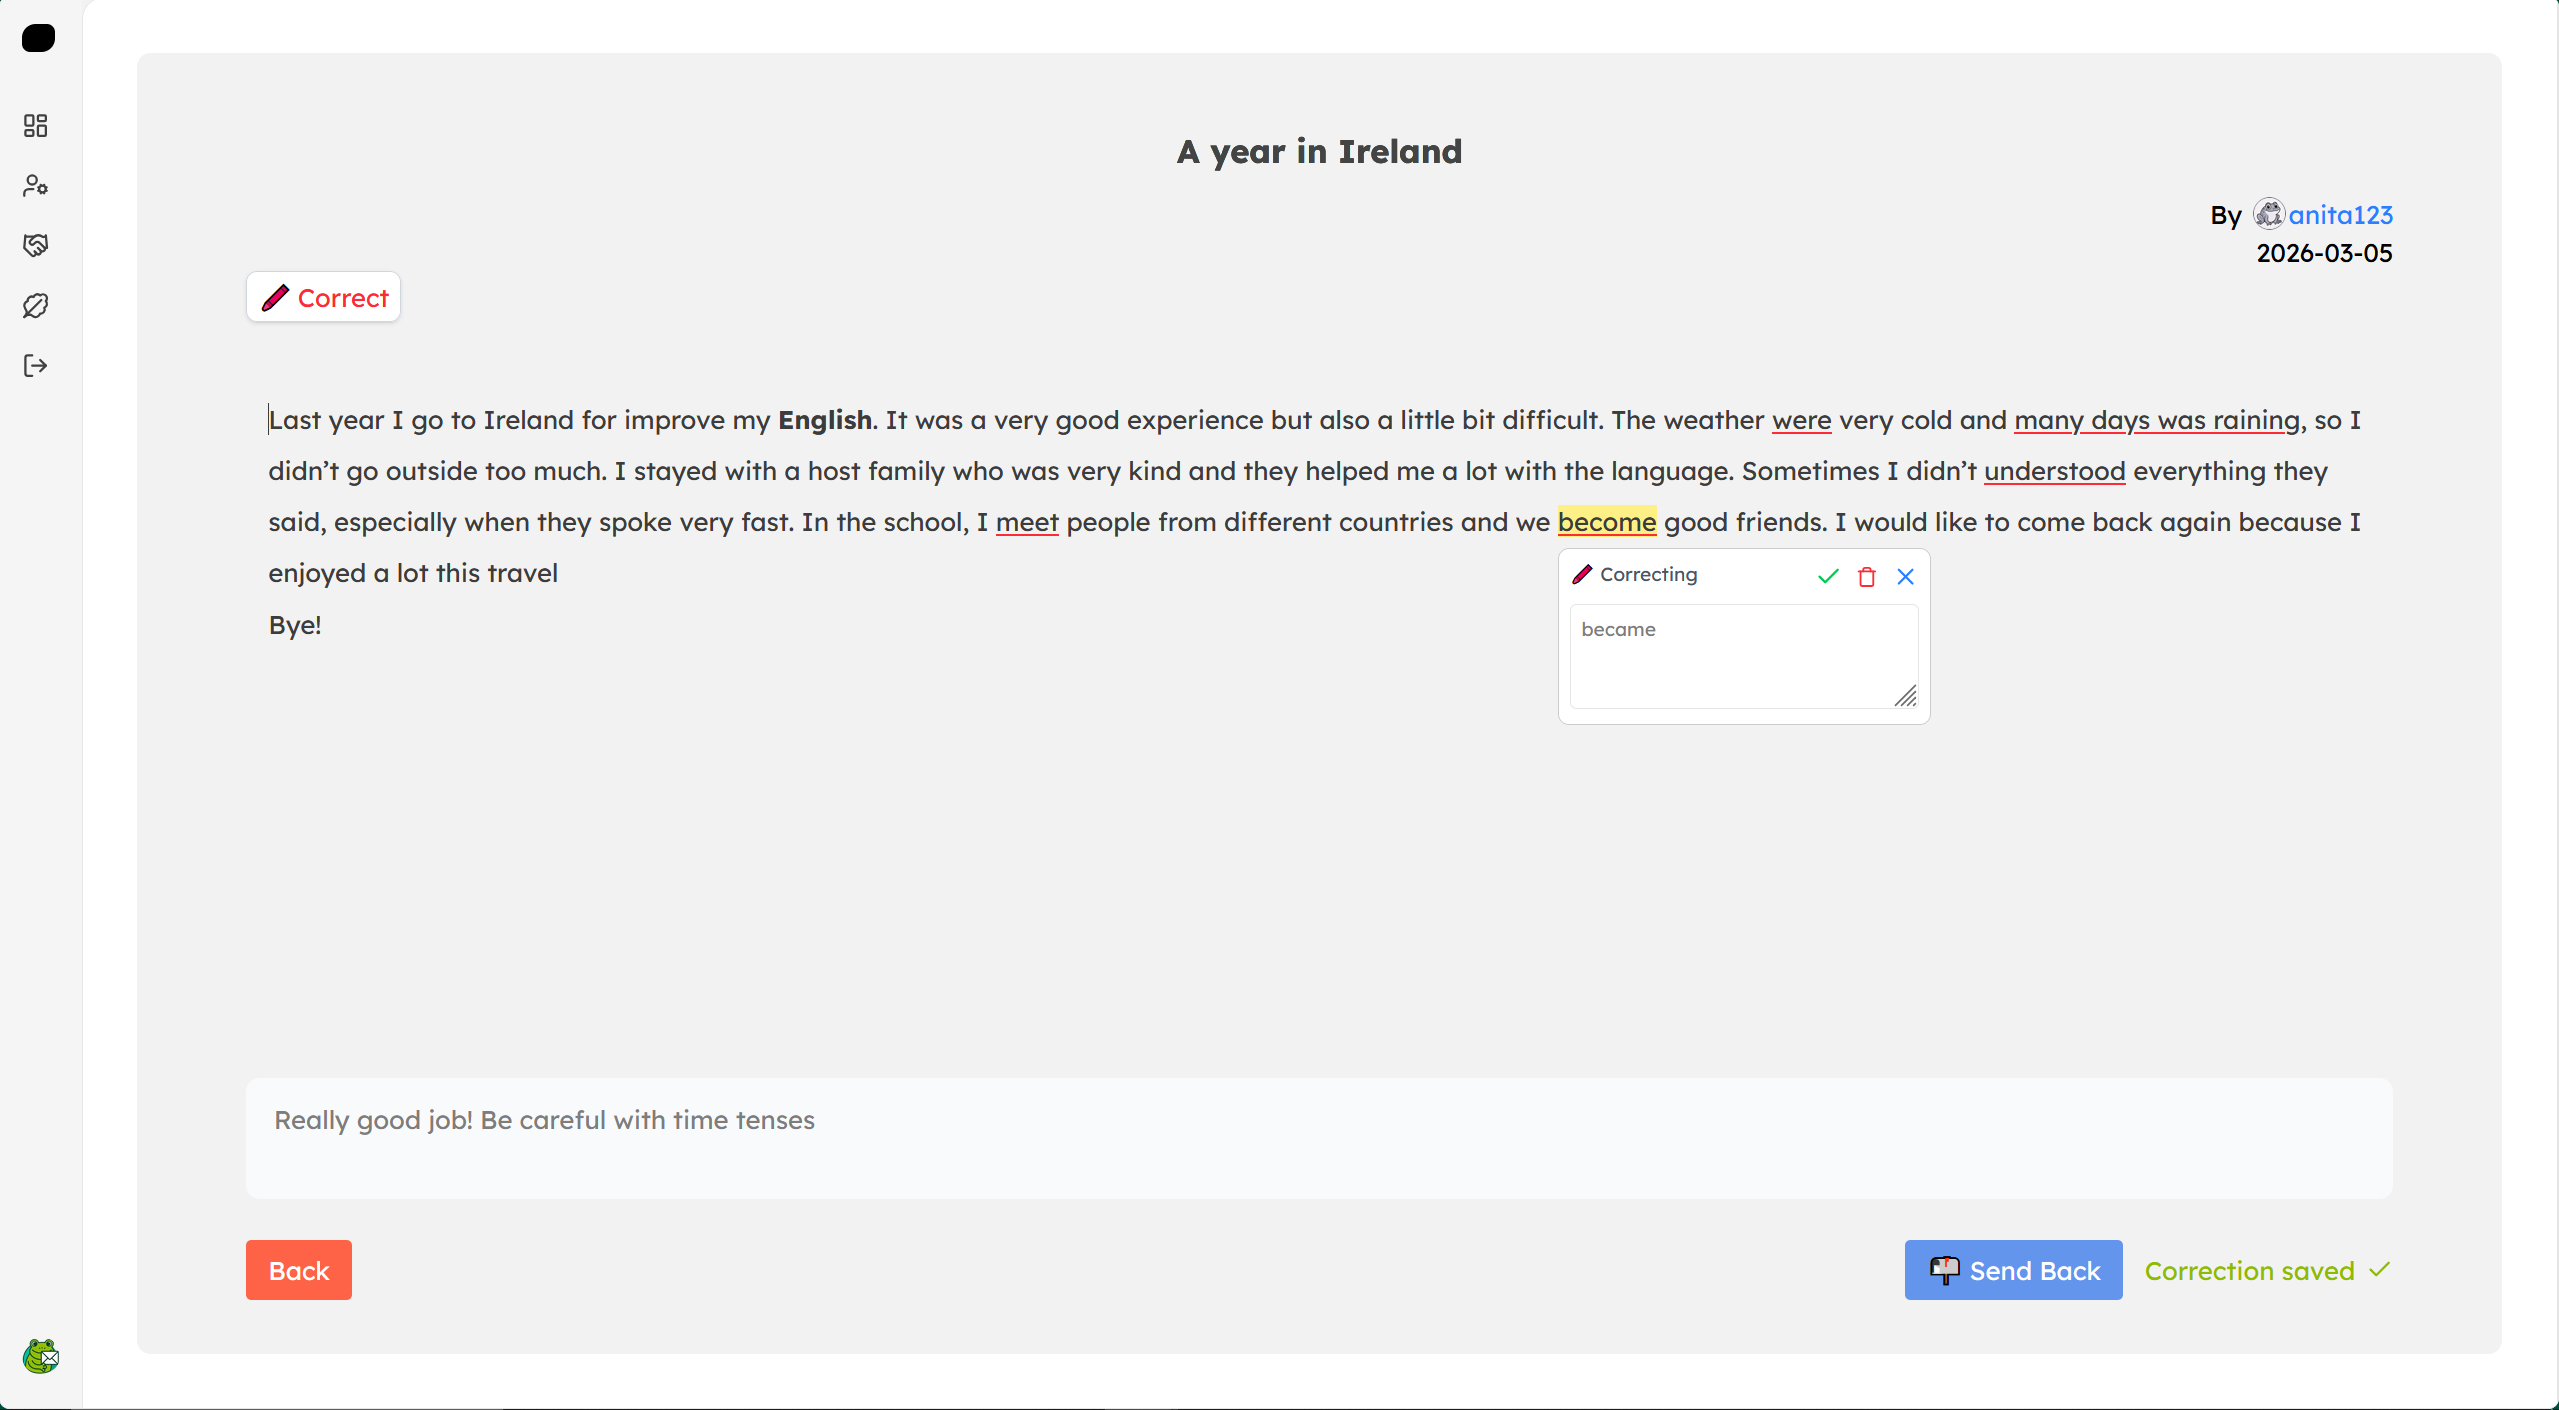
\includegraphics[width=\textwidth]{imagenes/ui/correct-letter2.png}
    \caption{Página de corrección de cartas}
    \label{fig:correct-letter}
\end{figure}

Esta página (\texttt{/correct-letter}) permite a los usuarios corregir las cartas escritas por otros en idiomas que dominan.

Para añadir correcciones, el usuario debe seleccionar fragmentos específicos del texto original que considere que contienen errores o se puede matizar. El texto seleccionado se resalta visualmente, y se abre un panel de escritura para asociarlo con una corrección sugerida o un comentario explicativo. Además de las correcciones específicas, el corrector puede dejar un comentario general sobre la carta al final.

El componente \texttt{TextCorrections} renderiza de forma dinámica el texto con las correcciones aplicadas. El proceso incluye:

\begin{enumerate}
    \item Parseo del texto original: Se divide el texto en fragmentos según las posiciones de corrección.
    \item Detección de solapamientos: Antes de añadir una nueva corrección, se verifica que no se solape con correcciones existentes mediante comparación de índices.
    \item Renderizado diferenciado: Cada fragmento se renderiza con estilos diferentes según sea texto sin corregir o texto corregido. Concretamente, el texto corregido va marcado en amarillo al hover y subrayado en rojo.
    \item Interactividad: Los fragmentos corregidos son interactivos. Al clicar en ellos o pasar el cursor, se abre un panel donde se pueden añadir o editar las correcciones.
\end{enumerate}

Para hacer esto posible, esta es la estructura de datos que se asocia a una corrección:

\begin{center}
\begin{minipage}{0.36\textwidth}
\begin{verbatim}
interface Correction {
    id: string;
    startIndex: number;
    endIndex: number;
    originalText: string;
    correctedText: string;
}
\end{verbatim}
\end{minipage}
\end{center}

\subsubsection{Página de Visualización de Correcciones Recibidas}

\begin{figure}[h]
    \centering
    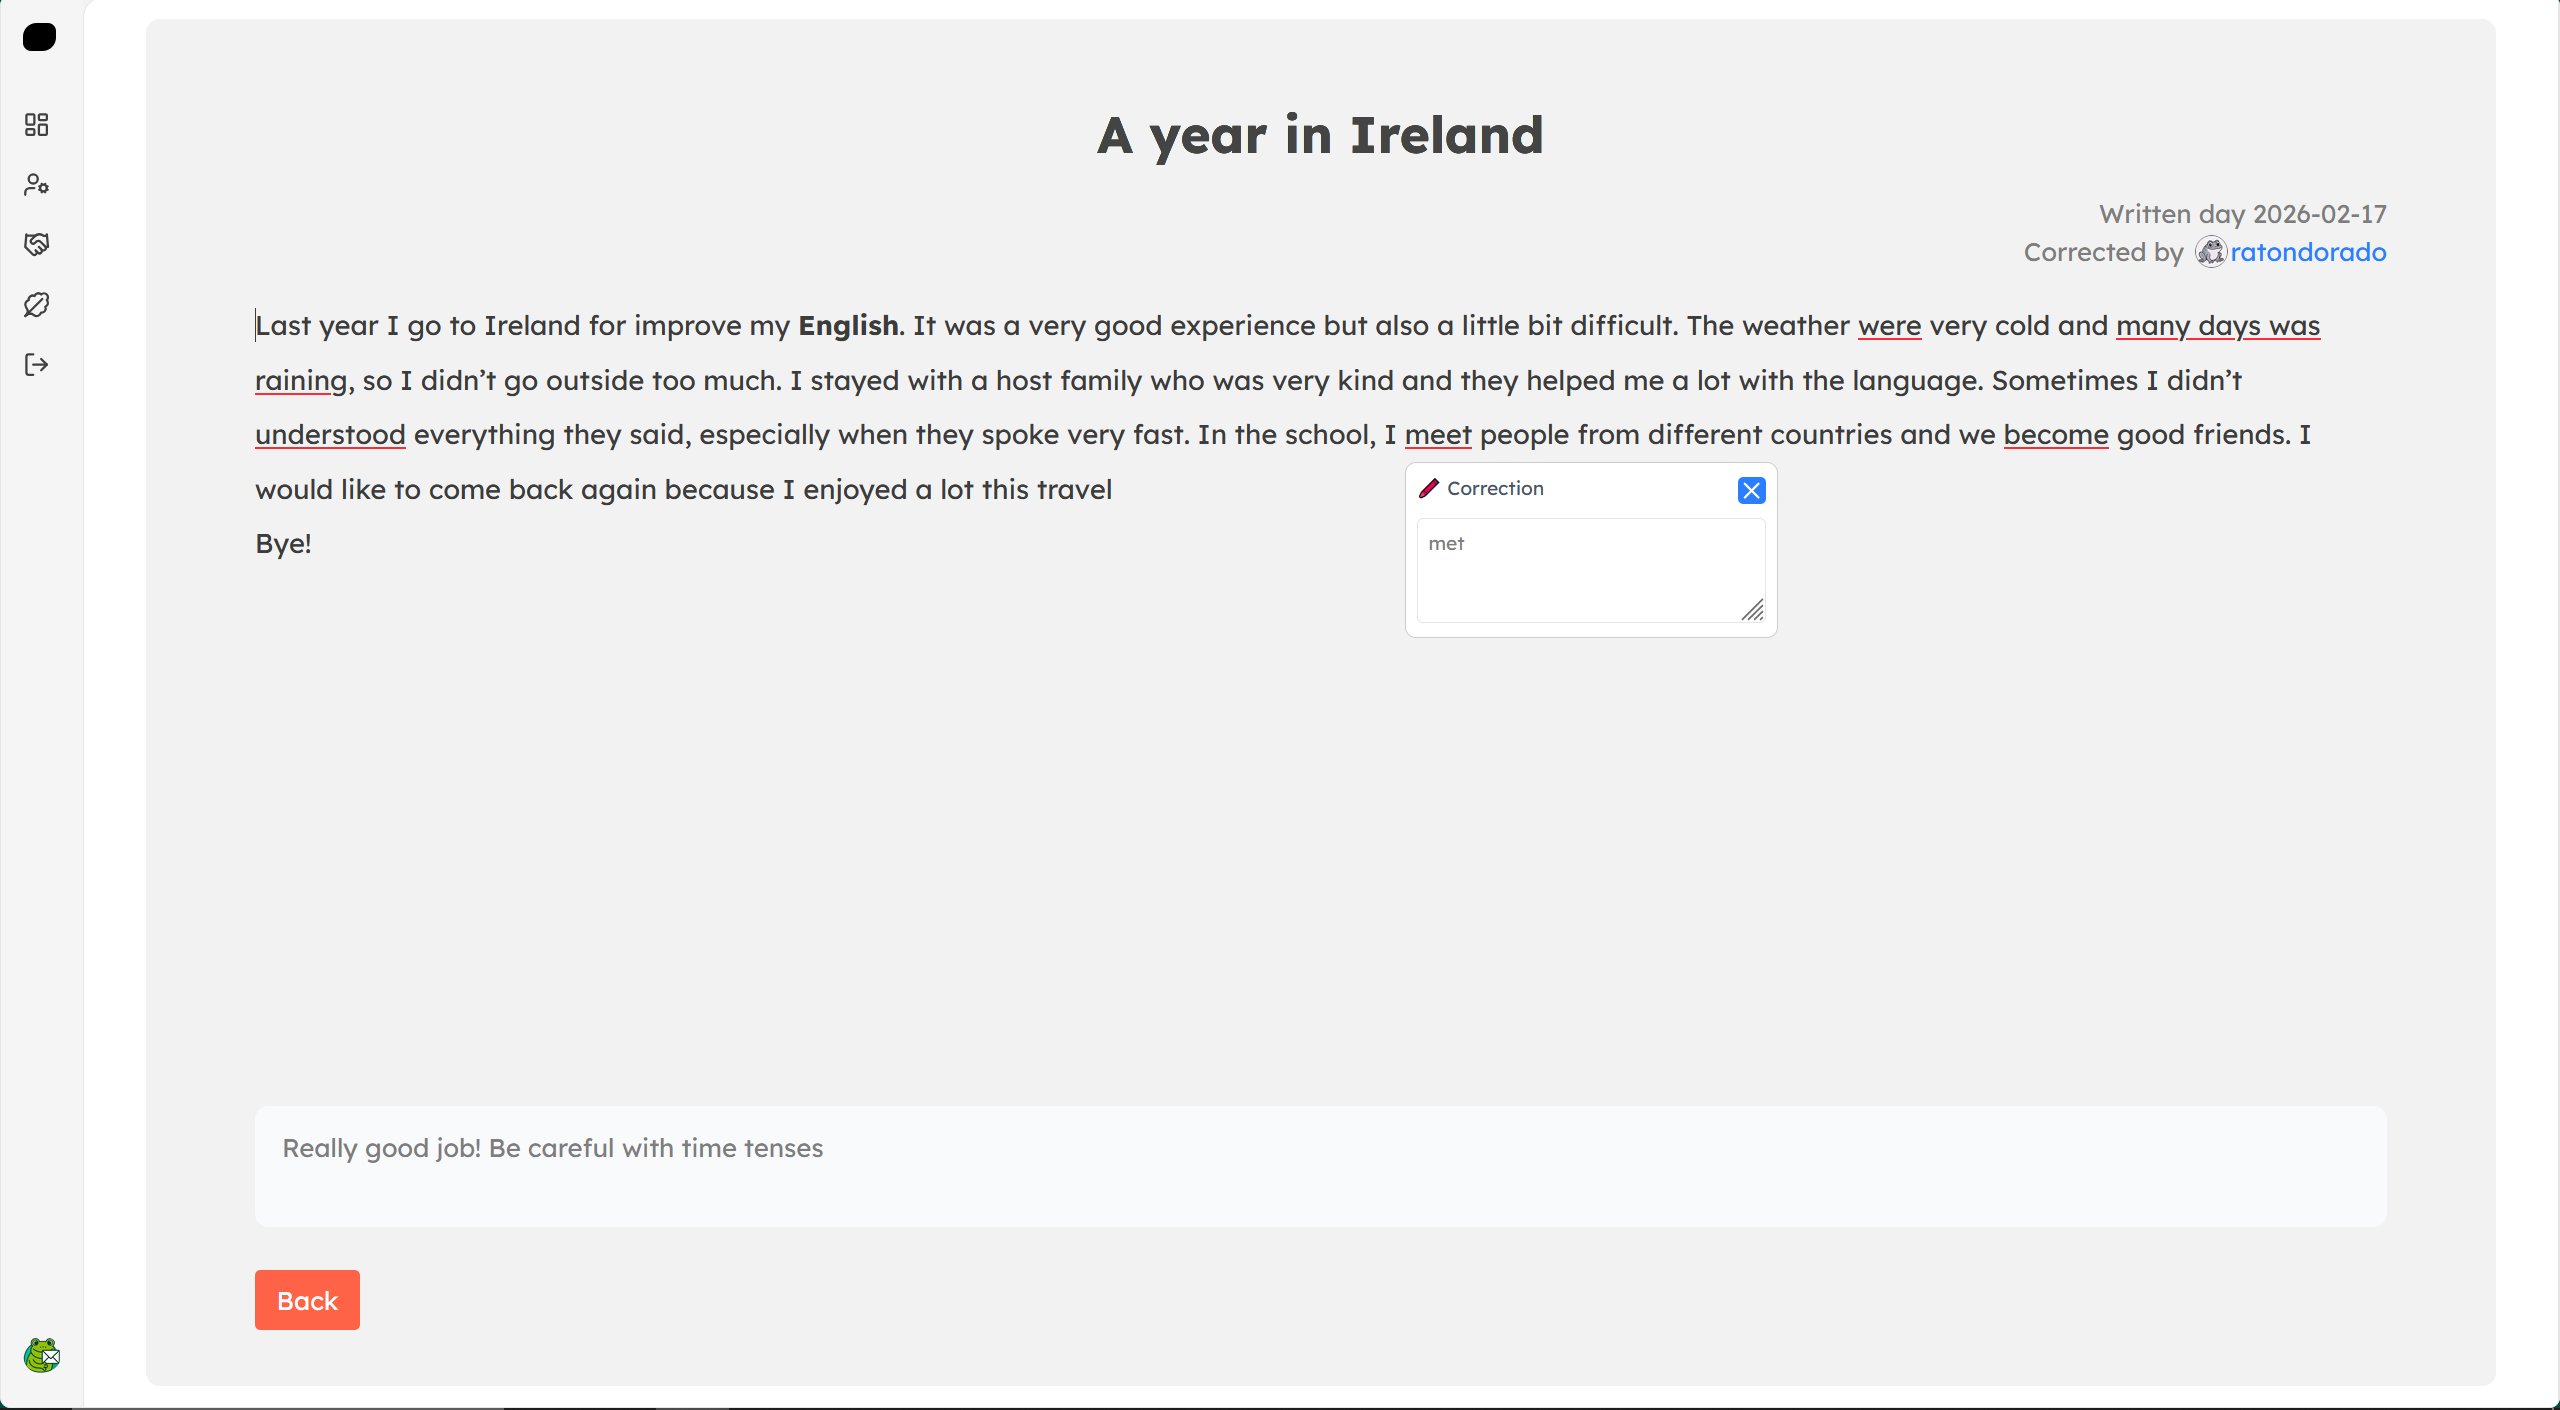
\includegraphics[width=\textwidth]{imagenes/ui/view-correction.png}
    \caption{Página de visualización de corrección recibida}
    \label{fig:view-correction}
\end{figure}

La página de visualización (\texttt{/view-correction}) de correcciones presenta al usuario remitente las correcciones recibidas en sus cartas. Esta interfaz permite al usuario aprender de sus errores de forma efectiva, clara y visualmente agradable. La interfaz es similar a la de Corrección de Cartas, pero sin permitir editar o enviar la corrección.

Se muestra el texto original con las secciones corregidas resaltadas en color diferenciado. Al hacer click o hover sobre una sección corregida, se muestra un panel con la corrección sugerida. Se muestran también los comentarios generales del corrector sobre la carta, y la información del corrector (nombre e imagen de perfil), que actúa como enlace a su página de perfil.

\subsubsection{Página de Amigos}

\begin{figure}[h]
    \centering
    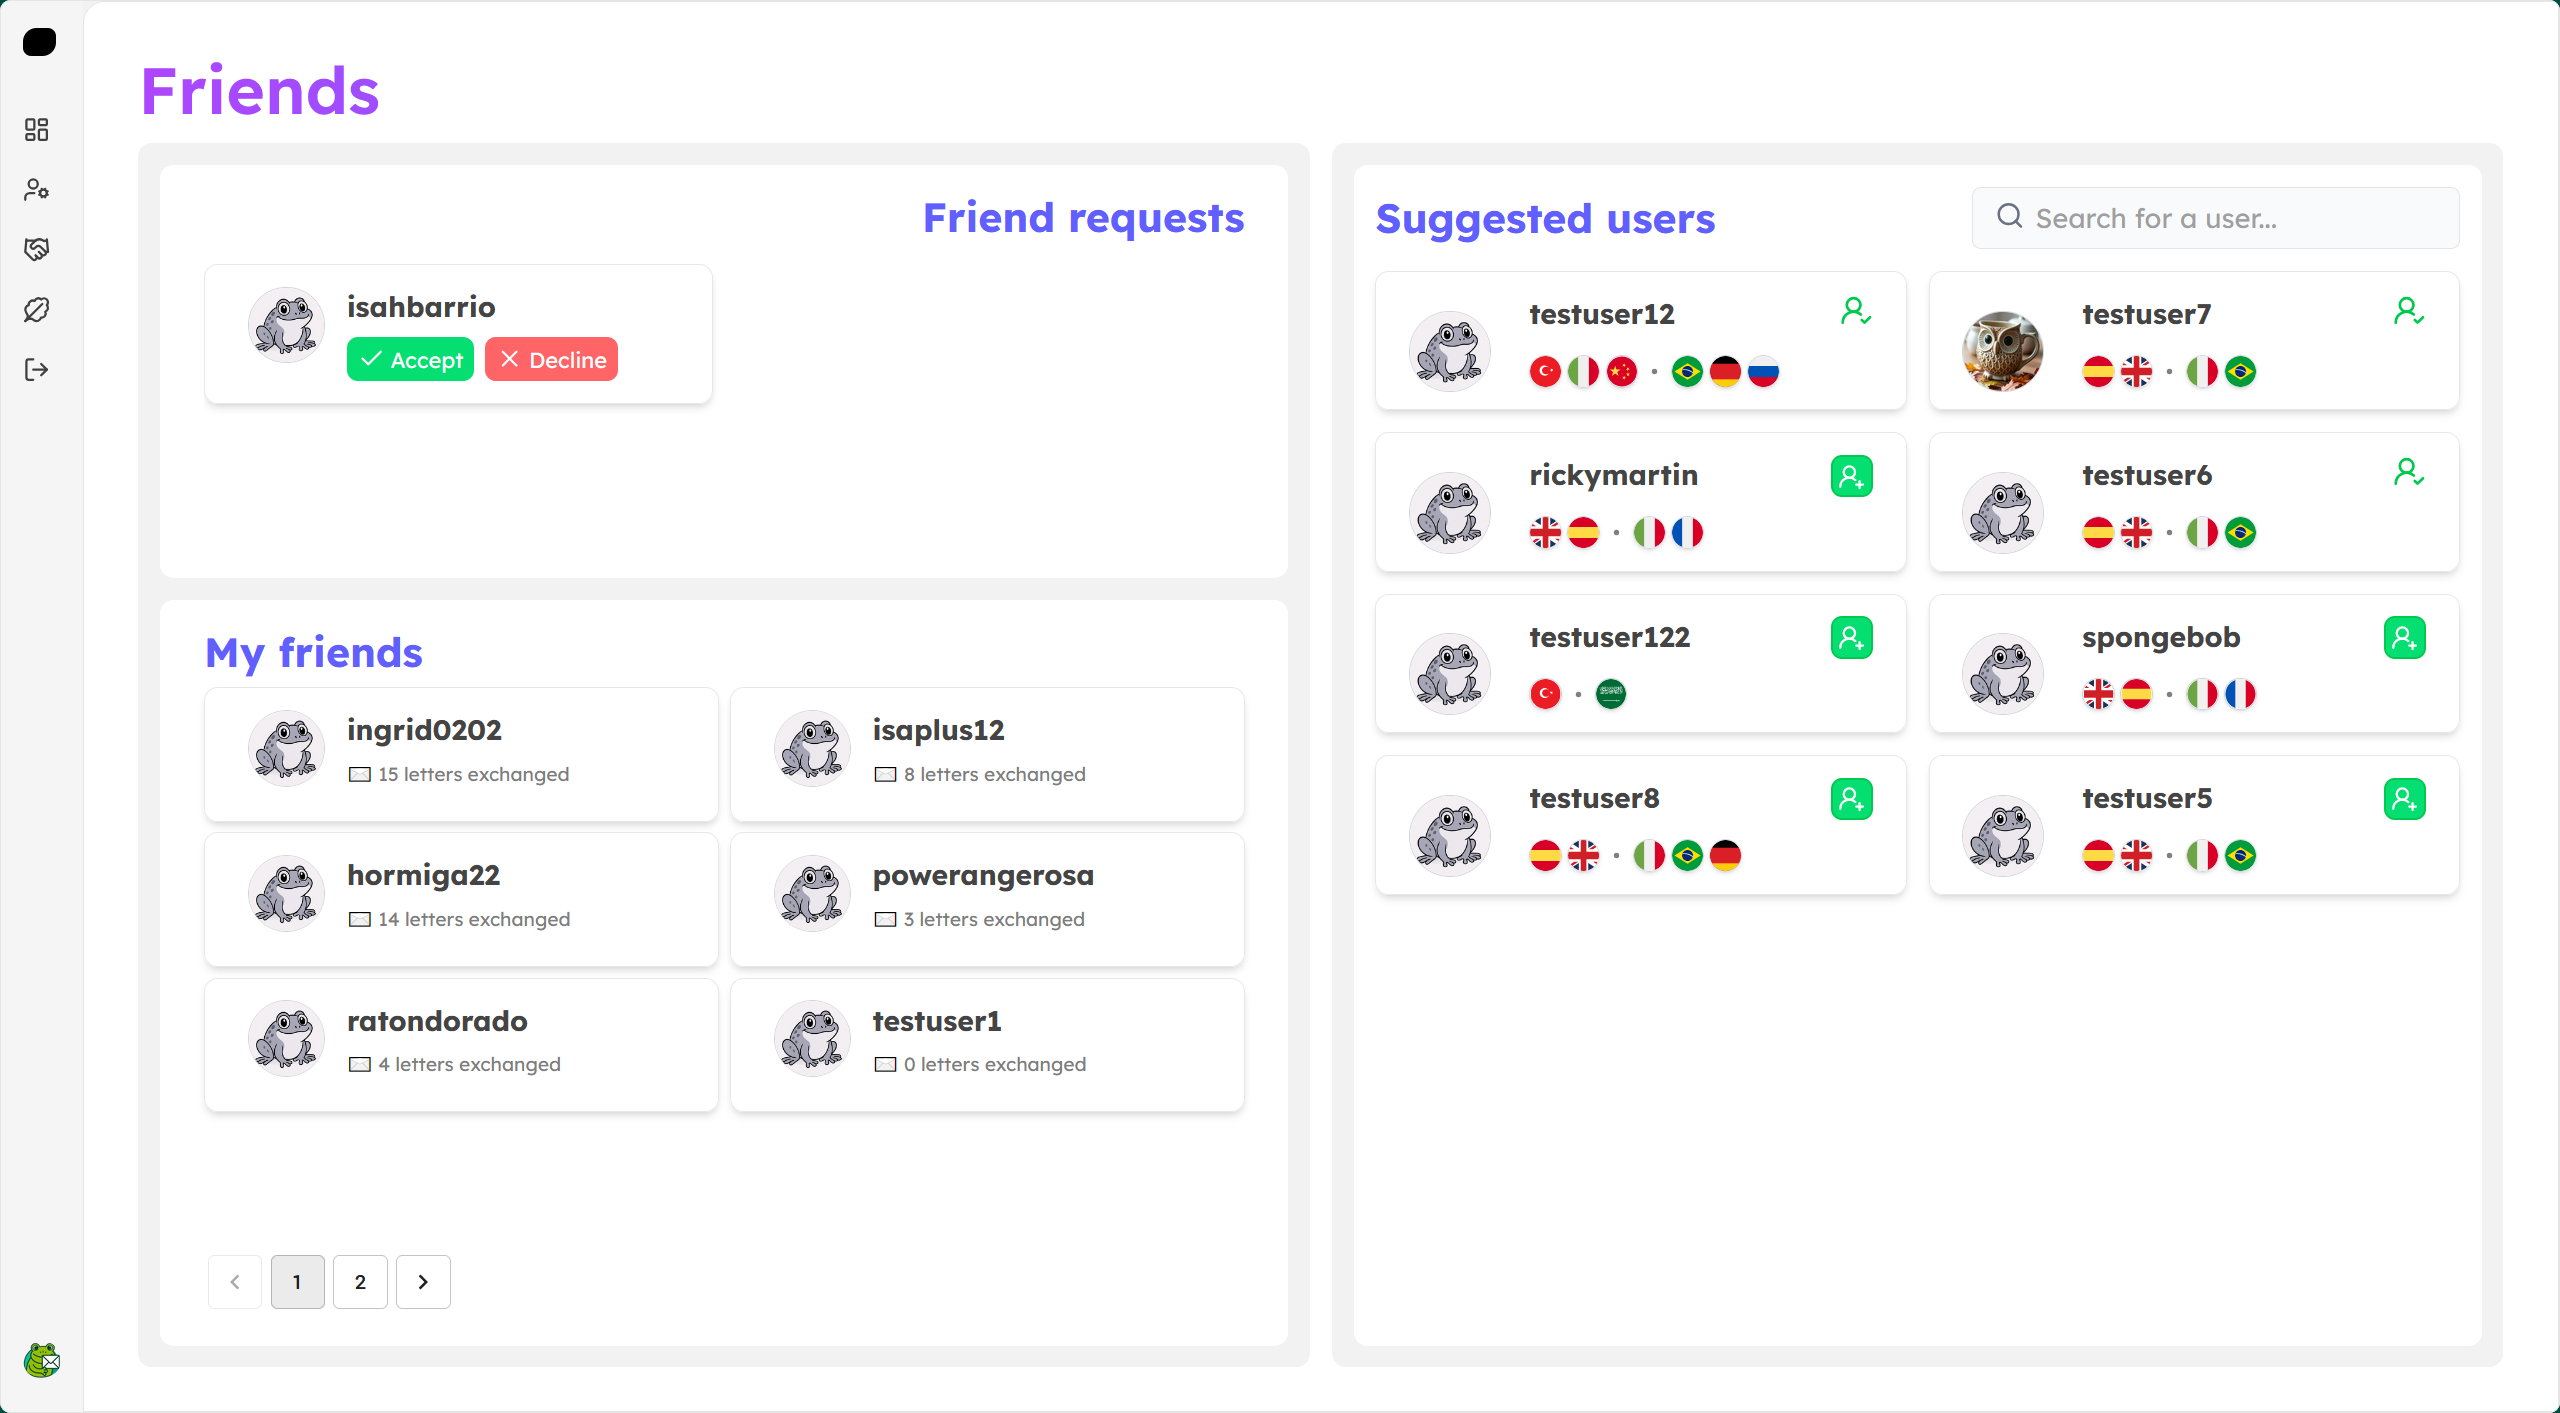
\includegraphics[width=\textwidth]{imagenes/ui/friends-page.png}
    \caption{Página de amigos}
    \label{fig:friends}
\end{figure}

En la página de amigos (\texttt{/friends}), el usuario puede gestionar las relaciones sociales dentro de la aplicación. Se divide en tres secciones:

\begin{enumerate}
    \item \textbf{Solicitudes de amistad}: Muestra las solicitudes pendientes recibidas, con opciones para aceptar o rechazar.
    \item \textbf{Lista de amigos}: Presenta las amistades establecidas con su avatar, nombre y estadísticas como el número de cartas intercambiadas.
    \item \textbf{Usuarios sugeridos}: Muestra usuarios recomendados basándose en idiomas en común, además de un buscador por nombre de usuario para poder encontrar un usuario en concreto que se desee agregar.
\end{enumerate}

La página implementa paginación para todas estas listas de usuarios y solicitudes. También, al clicar cualquiera de las tarjetas de usuario, se accede a la página de perfil de este.

\subsubsection{Página de Perfil de Usuario}

\begin{figure}[H]
    \centering
    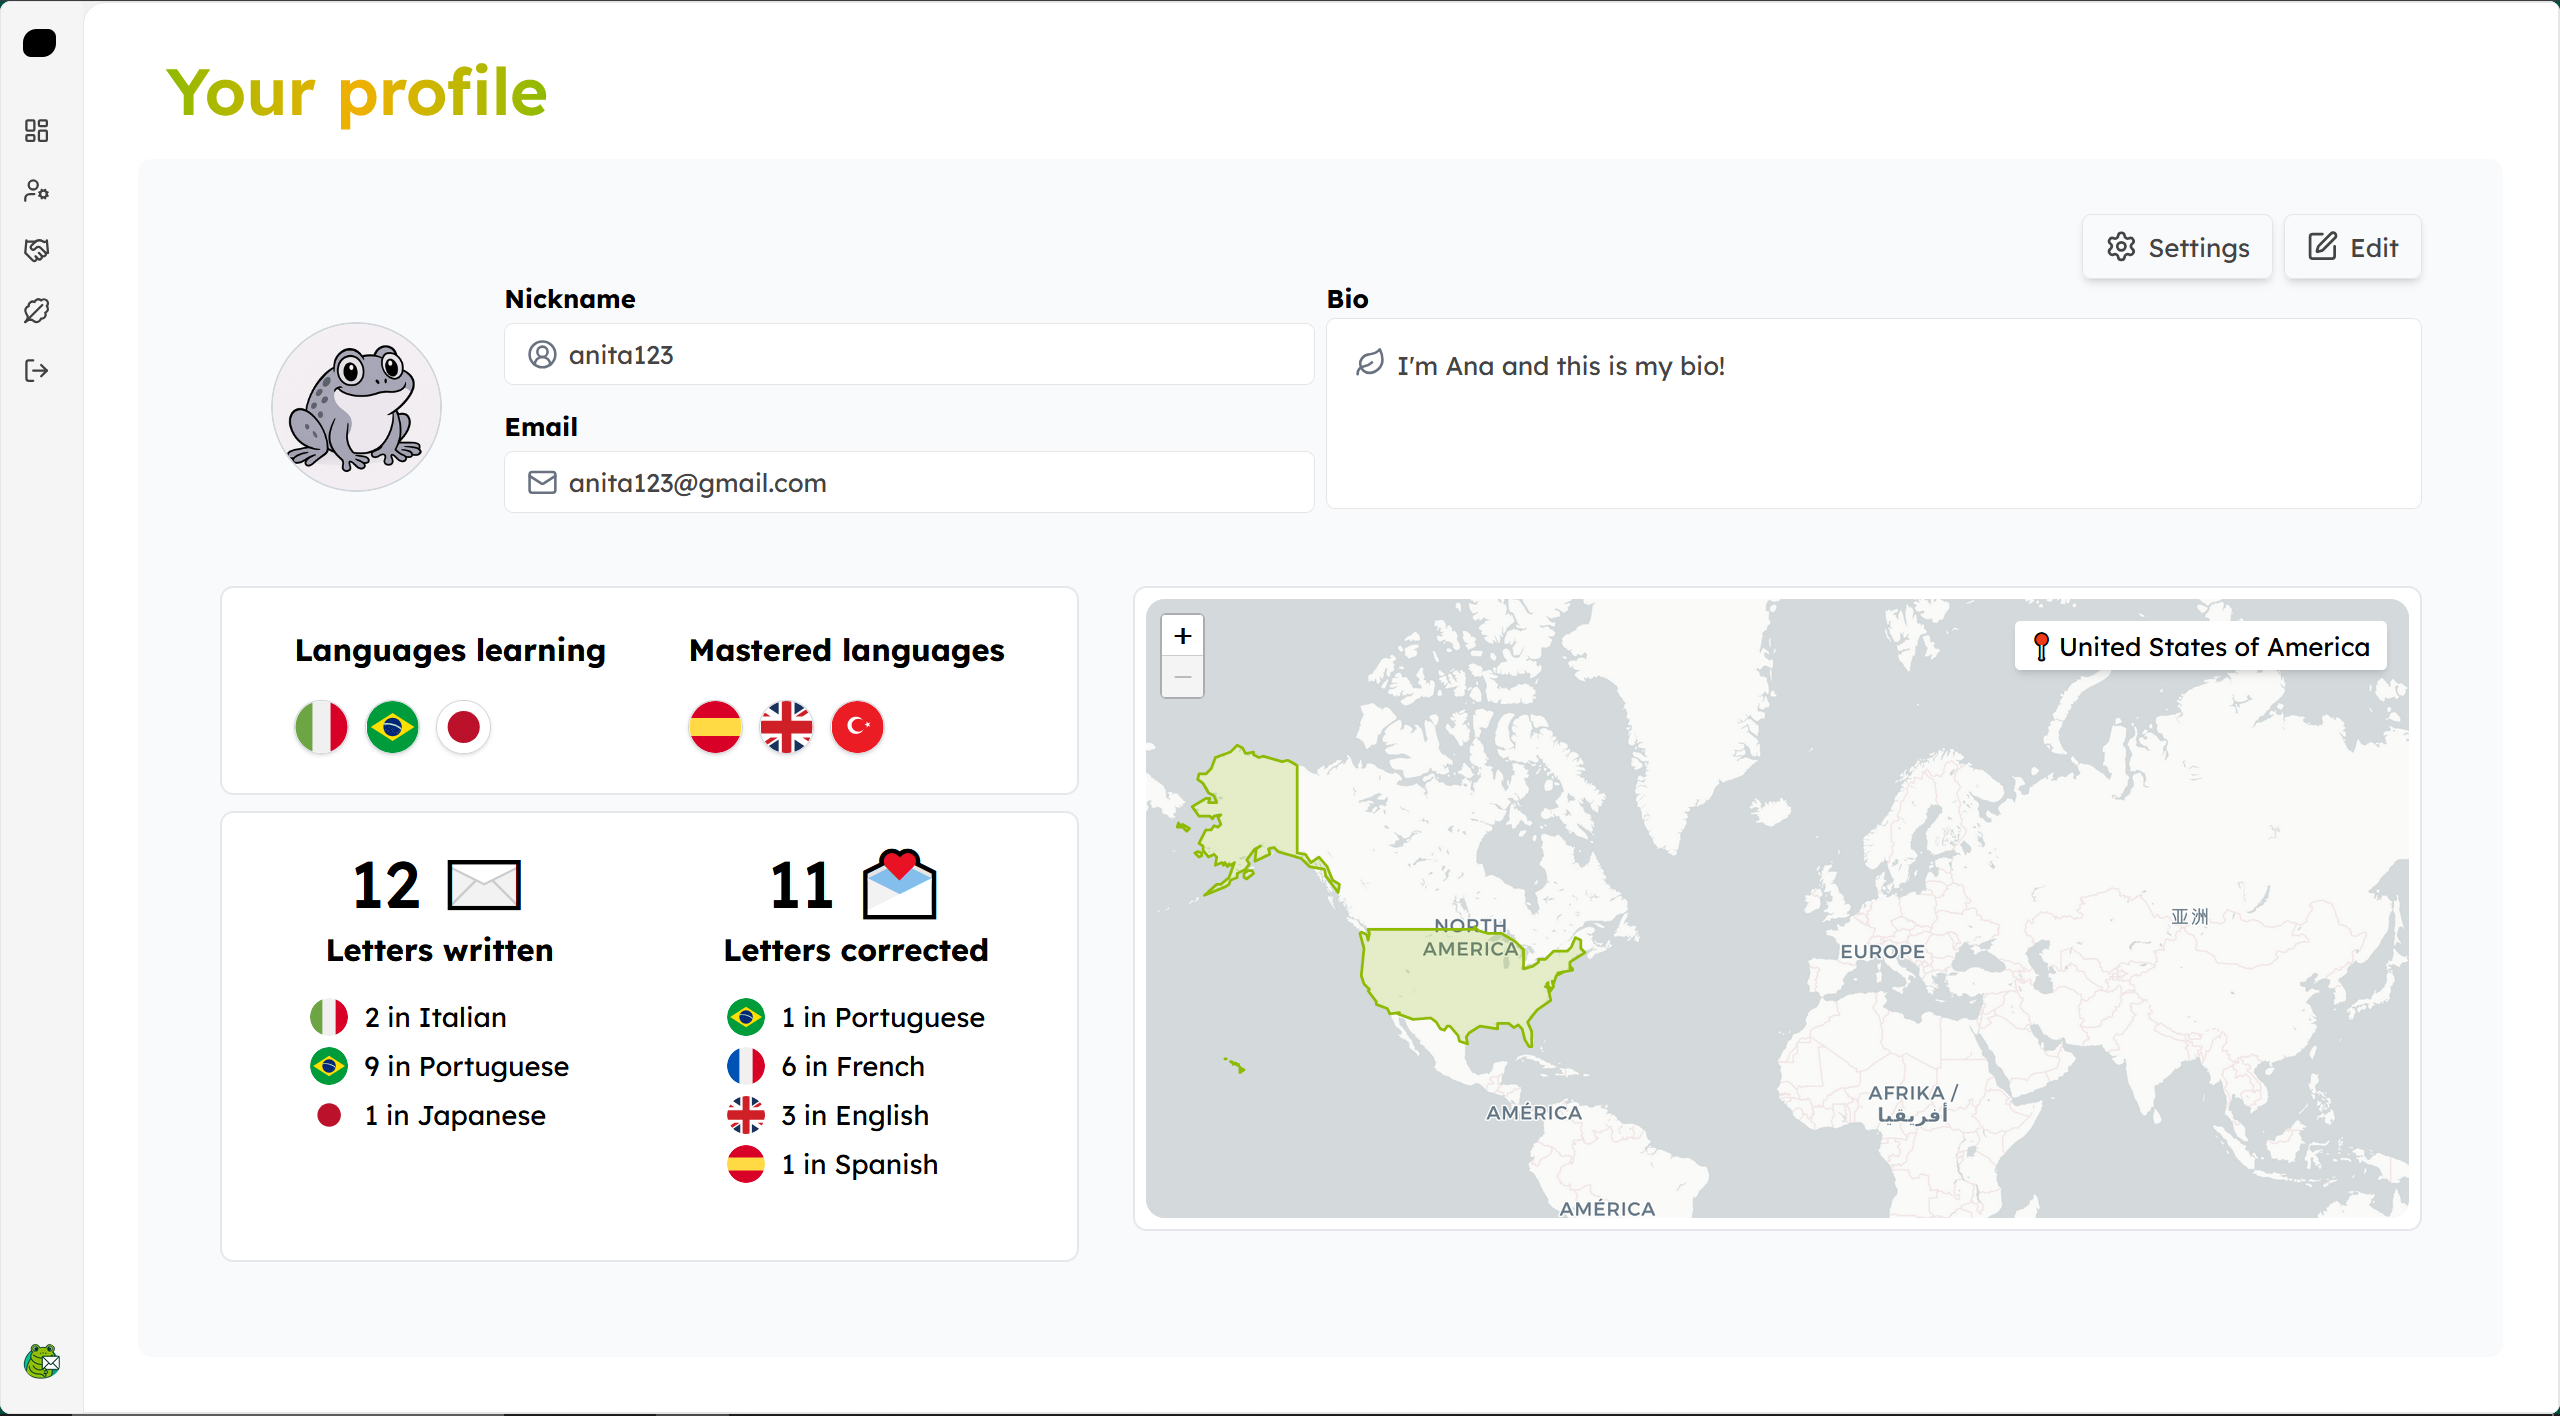
\includegraphics[width=\textwidth]{imagenes/ui/my-profile.png}
    \caption{Página de perfil de usuario}
    \label{fig:profile}
\end{figure}

La página de perfil muestra información detallada sobre un usuario. Se utiliza la misma página para el perfil propio y para el de otros usuarios. La página incluye:

\begin{itemize}[label={-}]
    \item Foto de perfil, nombre y biografía.
    \item Idiomas nativos y lenguas que está aprendiendo.
    \item Estadísticas de cartas escritas y corregidas en cada idioma.
    \item Ubicación geográfica visualizada en un mapa interactivo de React Leaflet.
    \item Para el perfil de usuario ajeno, un botón para dar la opción de eliminar de la lista de amigos en caso de tener a ese usuario agregado.
    \item Para el perfil de usuario autenticado (mi perfil), opciones de edición de la información del perfil y de configuración (cambiar contraseña o eliminar la cuenta).
\end{itemize}

\subsection{Técnicas de Optimización}

Finalmente, al igual que en el backend, en el frontend se han implementado varias técnicas de optimización. Estas técnicas se han aplicado de forma complementaria y selectiva, con el objetivo de mejorar el rendimiento de la aplicación y la experiencia de usuario en distintos niveles: carga de recursos, fluidez de la navegación, renderizado de componentes y comunicación con el backend.

\begin{enumerate}
    \item \textbf{Importaciones Dinámicas}: Componentes pesados como el mapa de la página de perfil se cargan dinámicamente solo cuando son necesarios. Esto es posible gracias a la función \texttt{dynamic} de Next.js, diseñada para optimizar el rendimiento mediante la técnica de carga diferida (\textit{Lazy Loading}) de los componentes, que asegura que el navegador descargue el código de estos componentes no al inicio sino en el momento en que los necesite. Mientras se carga, aparece un mensaje para informar al usuario del estado de carga.
    \begin{verbatim}
        const ImageUploader = dynamic(
            () => import("@/components/imageUploader"),
            { loading: () => <div>Loading...</div> }
        );
    \end{verbatim}

    \item \textbf{Memoización}: En la app se usan las funciones de React \texttt{useCallback} y \texttt{useMemo} para evitar recrear funciones y recalcular datos en cada renderizado.

    \item \textbf{Paginación}: Las listas de registros (cartas, correcciones, amigos) incluyen paginación para reducir la cantidad de datos cargados y renderizados simultáneamente. Se cargarán más elementos del servidor solo cuando el usuario lo solicite pasando de página en la lista.

    \item \textbf{Debouncing}: En campos de búsqueda y filtrado, se implementa debouncing para reducir el número de llamadas a la API, como se ha descrito en la sección anterior de arquitectura del backend.

    \item \textbf{Lazy Loading de imágenes}: Las imágenes de perfil se cargan de forma diferida para mejorar el tiempo de carga inicial.

    \item \textbf{Pantallas esqueleto}: Para mejorar la experiencia del usuario durante la carga de datos, se han utilizado pantallas esqueleto (\textit{skeleton screens}). Se genera una estructura visual gris translúcida que replica la de la página real (títulos, bloques de contenido, botones...) mientras se cargan los datos del servidor. Esto reduce la sensación de espera porque el usuario ya ve dónde aparecerá cada elemento. Una vez que los datos llegan, el esqueleto se reemplaza con el contenido definitivo.

    \begin{figure}[H]
        \centering
        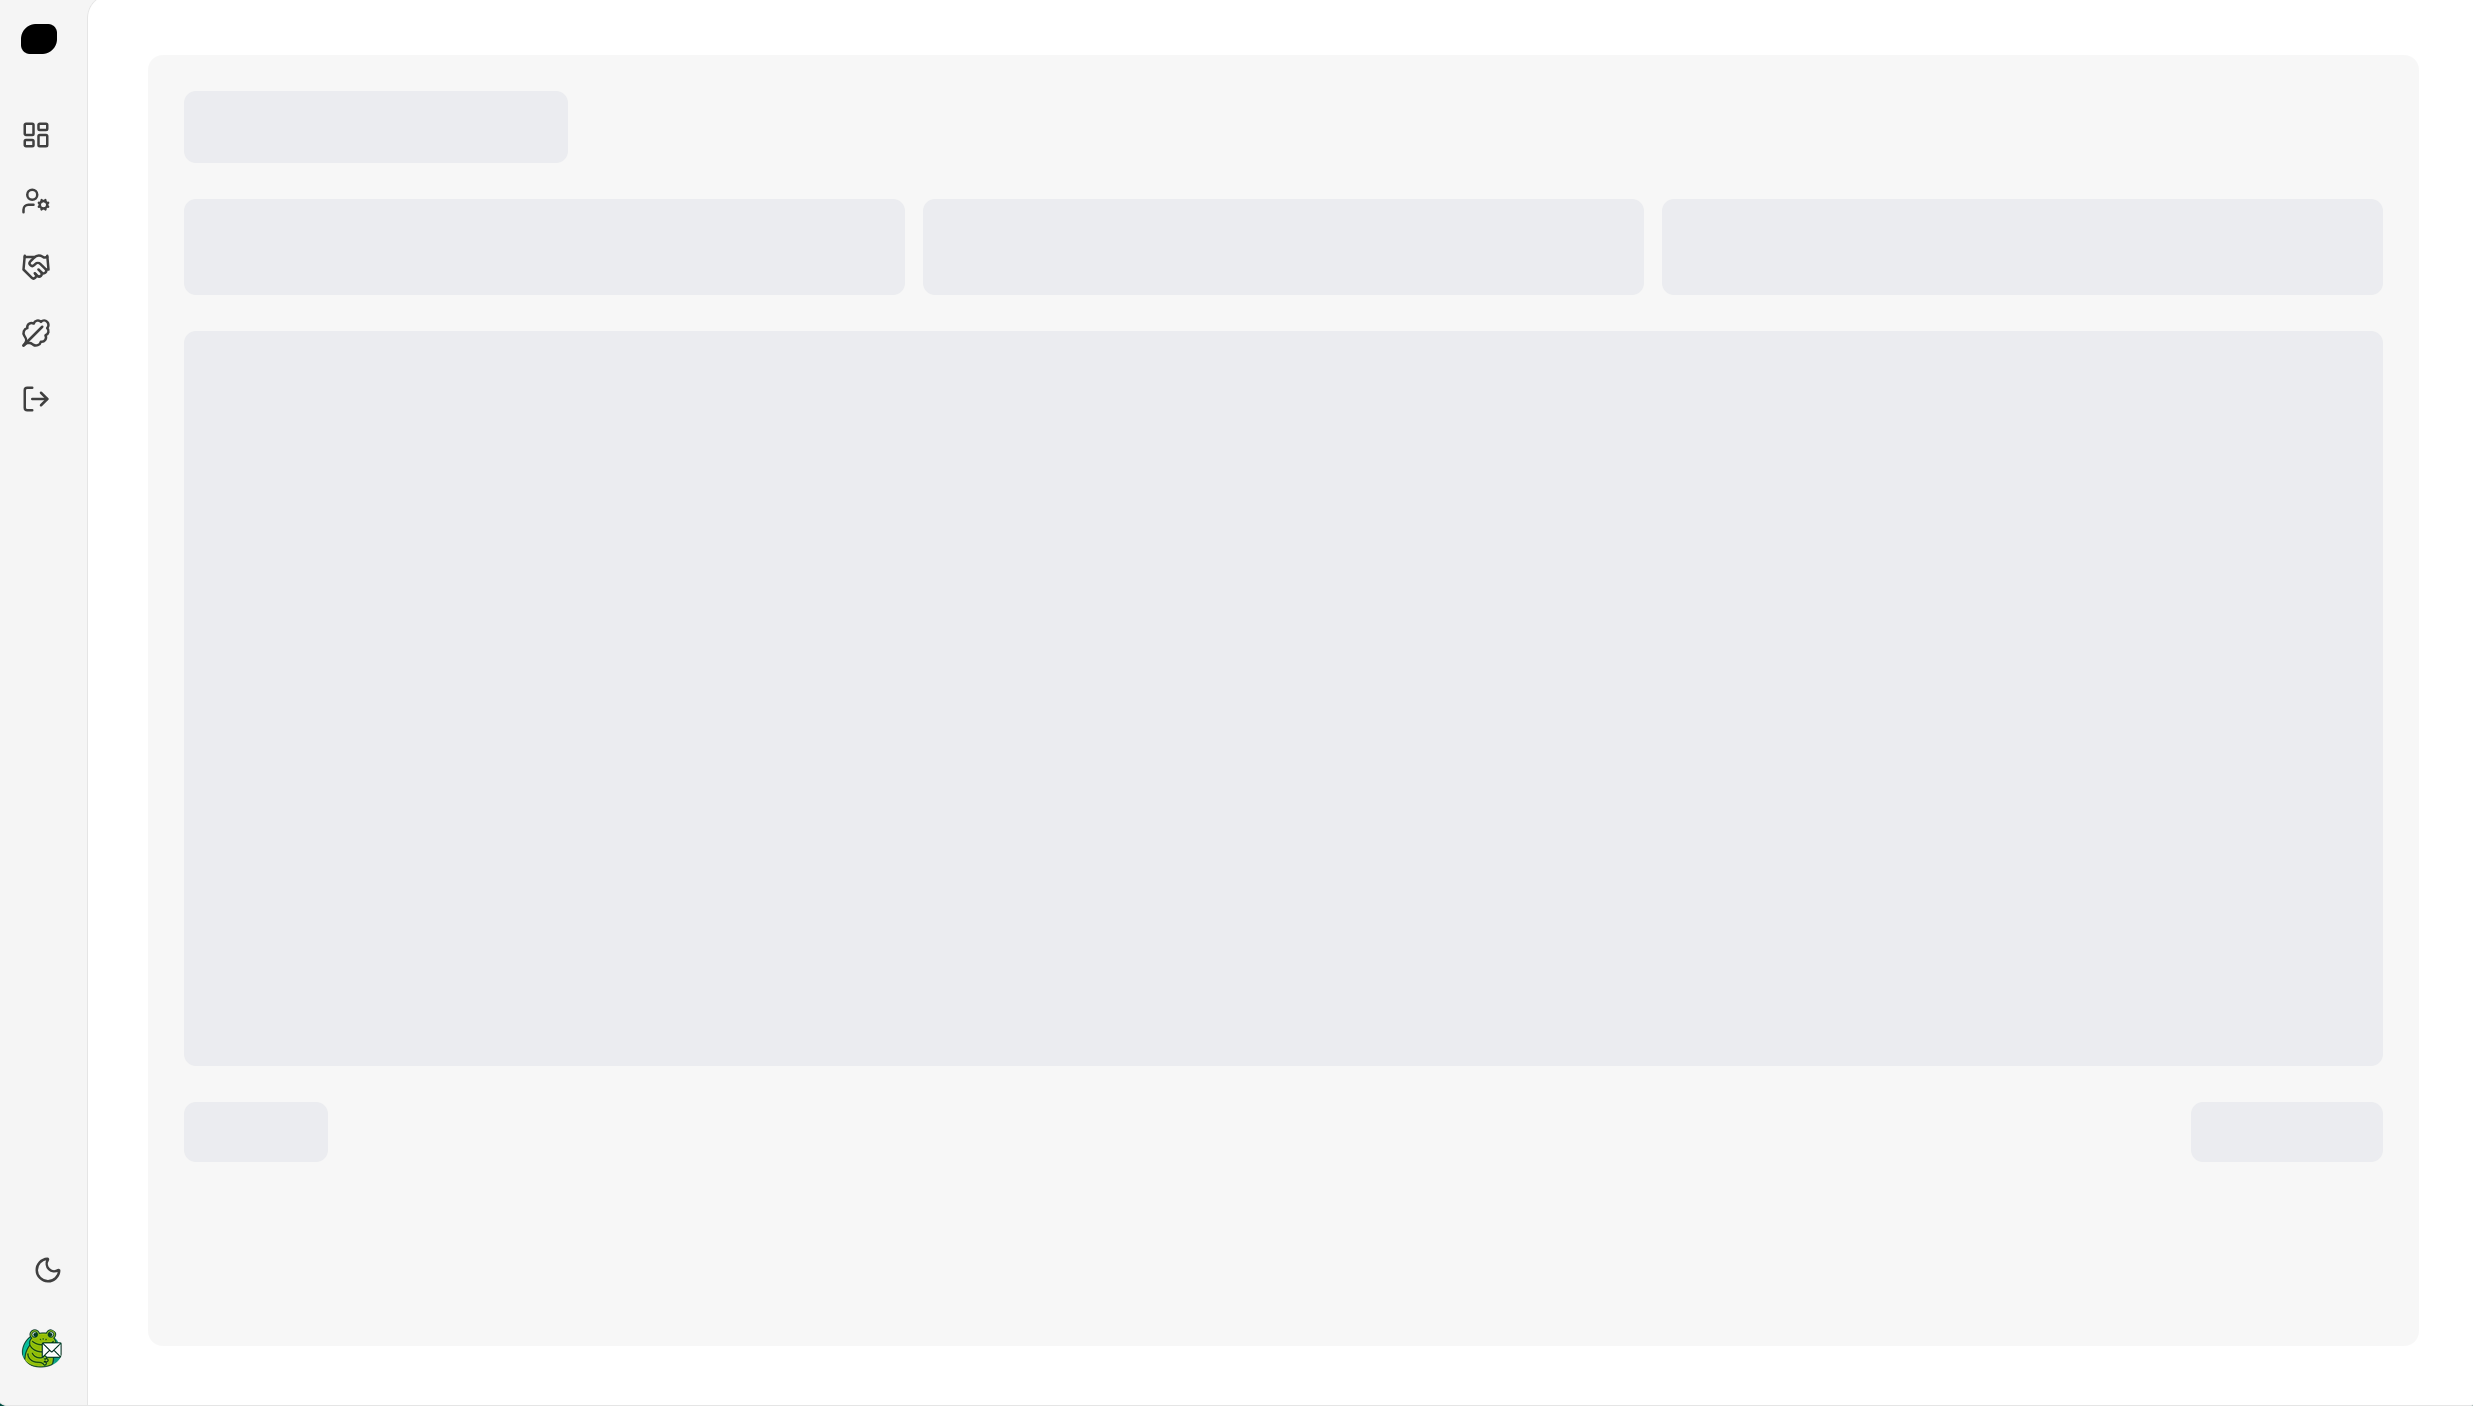
\includegraphics[width=\textwidth]{imagenes/ui/skeleton.png}
        \caption{Ejemplo de Pantalla Esqueleto}
        \label{fig:skeleton}
    \end{figure}
\end{enumerate}

